\begin{headerBlock}
\chapter{Conductimétrie}
\label{LC_Conductimétrie}
 \end{headerBlock}

%%%%%%%%%%%%%%%%%%%%%%%%%%%%%%%%%%%%%%%%%%%%%%%%%%%%
%%%% Références


%%%%%%%%%%%%%%%%%%%%%%%%%%%%%%%%%%%%%%%%%%%%%%%%%%%%
%%%% Plan
\begin{reportBlock}{Bibliographie}

\begin{center}
\begin{tabular}{|c|c|c|c|}\hline
Titre & Auteur(s) & Editeur (année) & ISBN \\ \hline
PC Tout-en-un MPSI ~ & Bruno FOSSET,  ~ & Dunod  ~ & ~ \\
~ & Jean-Bernard BAUDIN, ~ &  ~ & ~ \\
~ & Frédéric LAHITÈTE  ~ &  ~ & ~ \\ \hline
Ressources en ligne & ~ & Eduscol & ~ \\ \hline
\end{tabular}
\end{center}

\end{reportBlock}

\begin{reportBlock}{Plan détaillé}

\underline{Niveau} : Tle STL - SPCL \\

\underline{Pré-requis} :
\begin{itemize}
\item Loi d'Ohm
\item Dosage
\item Solubilité/précipitation
\end{itemize}


\section*{Introduction pédagogique}

Leçon placée en début d'année de terminale.

\paragraph*{Prérequis}
\begin{itemize}
\item Loi d'Ohm
\item Dosage
\item Solubilité / Précipitation
\end{itemize}

\paragraph*{Notions importantes}

\begin{itemize}
\item Conductance/conductimétrie.
\item Electrolyte.
\item Loi de Kohlrausch.
\item Prévoir l'allure de titrage.
\end{itemize}

\paragraph*{Objectifs}

\begin{itemize}
\item Principe du conductimètre.
\item Loi de Kohlrausch.
\item Titrage par conductimétrie.
\end{itemize}

\paragraph*{Difficultés}

\begin{itemize}
\item Beaucoup de grandeurs différentes avec différentes unités : conductance, conductivité (Siemens).
\item Cellule conductimétrique (vs. électrodes connues) et fonctionnement du conductimètre.
\item Ions mobiles qui conduisent en solution.
\item Prévoir l'allure $\sigma(V)$ (méthode du tableau)
\end{itemize}

\section*{Introduction}

\textbf{Question:} Quelle est la condition pour qu'une solution conduise le courant ?

\paragraph*{Manipulation qualitative:} Solution d'eau distillée dans laquelle on fait passer le courant d'une pile reliée à une ampoule (ou une LED) : l'ampoule ne s'allume pas. Elle s'allume si on rajoute du sel (cf. exp 1).

\section{Conductance et conductivité}

\subsection{Définitions}

\paragraph*{Electrolyte} Solution capable de conduire le courant en présence d'ions mobiles. \\
ex: eau salée \ce{Na^+} et \ce{Cl^-}.

\paragraph*{Conductance} $G = \frac{1}{U} = \frac{1}{R}$. Unité : $S = \Omega^{-1}$ (Siemens). Cette grandeur n'est pas intrinsèque à la solution.

\subsection{Présentation du condcutimètre}

\paragraph*{Conductivité} Schéma de fonctionnement d'un conductimètre : une \textbf{cellule conductimétrique} constituée de deux plaques parallèles de surface immergée $S$ et séparées d'une distance $L$. \\

\paragraph*{Conductivité}: $\sigma = \frac{G L}{S}$ en $S.m^{-1}$, avec $S$ la surface d'une plaque de la cellule conductimétrique et $L$ la distance entre les deux plaques.


\subsection{Facteurs d'influence de la conductivité (16')}

\paragraph*{Manipulation: } Mesure de la conductivité de deux solutions (NaCl et KCl) (cf. exp 2). $\sigma(_ce{KCl}) = 10,32~mS.cm^{-1}$ et $\sigma(\ce{KCl}) = 12,17~mS.cm^{-1}$

- $\sigma$ dépend de la nature des ions mobiles. \\
- $\sigma$ dépend de la température.\\
- $\sigma$ dépend de la concentration des ions présents en solution.

\subsection{Loi de Kohlrausch (19')}

Soit $n$ ions présents dans un électrolyte, on a 
\begin{equation}
\sigma(T) = \sum_i z_i \lambda_i^0(T) C_i
\end{equation}
avec : \\
$z_i$ le nombre de charge de l'ion $i$, ex: z(\ce{Na^+}) = 1, z(\ce{Cl^{-1}}) = 1. \\
$C_i$ la concentration de l'ion $i$ en $mol.L^{-1}$  \\
$\lambda_i^0(T)$ la conductivité molaire ionique \color{purple} \underline{à dilution infinie} \color{black} de l'ion $i$ en $S.m^2.mol^{-1}$. Elles sont tabulées à 25°C.


\section{Application : titrage par précipitation (24'50)}
cf. exp 3. \\

$ \ce{Cl^{-1}_{(aq)}} + \ce{Ag^+_{(aq)}} = \ce{AgCl_{(s)}}$ . Constante d'équilibre : $K = \frac{1}{K_s} = 10^{9.8} \gg 1$.

\subsection{Analyse qualitative}

Tableau de réaction qualitatif. Avant l'équivalence : \ce{Na^+} reste constante, \ce{Cl^{-}} diminue, \ce{NO_3^{-}} augmente, \ce{Ag^+} disparaît. Comme $\lambda^0(\ce{Cl^{-1}}) > \lambda^0(\ce{NO_3^{-1}})$, la conductivité diminue. Après l'équivalence: \ce{Na^+} reste constante, \ce{Cl^{-}} a disparu, \ce{NO_3^{-}} augmente, \ce{Ag^+} augmente. Comme $\lambda^0(\ce{Cl^{-1}}) > \lambda^0(\ce{NO_3^{-1}})$, la conductivité augmente.

\subsection{Détermination de la concentration en ions chlorure dans le sérum physiologique}

  %\begin{figure}[!htbp]
  \begin{center}
   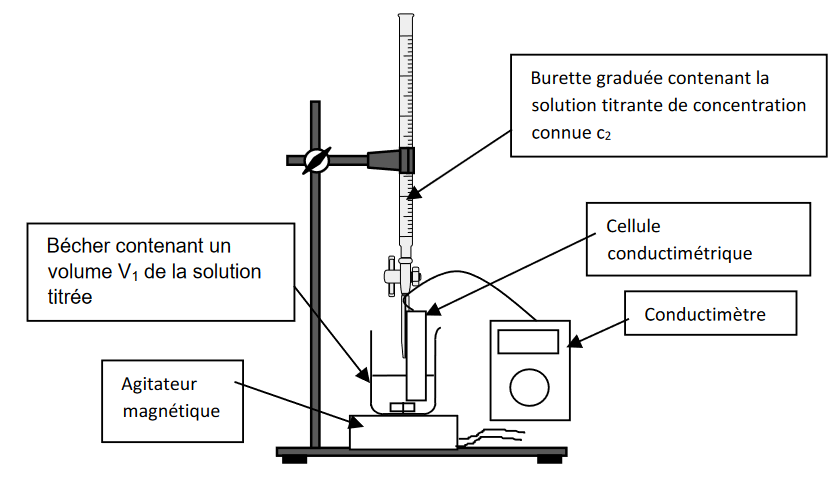
\includegraphics[scale=0.5]{Leçon_chimie/LC_SPCL/LC_Conductimetrie/Schema_titrage.png}
  \end{center}
 
  %\caption{\label{fig:localisation}Schéma de principe du titrage conductimétrique. Le solution titrante est une solution de $AgCl$ à $0.2 mol/L$. La solution titrée est du sérum physiologique.}
  %\end{figure}


Courbe $\sigma(V)$. La détermination du volume équivalent permet de remonter à la concentration des ions Cl$^-$.

\section{Conclusion} Application titrage pour sonder la qualité de l'eau.

\end{reportBlock}

\begin{reportBlock}{Questions posées}

\begin{itemize}

\item Est-ce que c'est important de connaître la valeur du volume d'eau ajouté dans le bécher contenant le réactif titrant lors du titrage conductimétrique ? \textcolor{purple}{Non, ce n'est pas important pour déterminer le volume équivalent lors du titrage.}

\item Pourquoi diluez-vous ?  \textcolor{purple}{Pour pouvoir s'affranchir de la dilution, i.e. obtenir des courbes affines de $\sigma(V)$. Si la solution n'est pas assez dilué on obtient des branches d'hyperbole, qu'on peut corriger en représentant non pas la conductivité $\sigma$ mais la conductivité corrigée $\sigma_{cor}=\sigma \times \frac{V_{tot}}{V_0}$. D'autre part, ça permet d'avoir assez d'eau pour y immerger l'électrode.}

\item Le point à $1mL$ dévie de la droite, pourquoi ? \textcolor{purple}{Cela peut être dû au fait qu'à ce volume, on n'est pas forcément dans le régime linéaire de la loi de Kohlrausch.}

\item Vous donner comme exemple le titrage des ions nitrate. Comment proposez-vous d'en déterminer la concentration ? \textcolor{purple}{En réalisant le même titrage que pour les ions chlorure.} Peut-on dans ce cas déterminer séparément la concentration des 2 analytes (\ce{NO_3^-} et \ce{Cl^-}) ? \textcolor{purple}{Non.}

\item Qu'est-ce qu'on peut chercher d'autre dans l'eau ? Les organismes vivants dans l'eau en ont besoin. \textcolor{purple}{Oxygène.} Comment le titrer ? \textcolor{purple}{Titrage par la méthode de Winkler.} Quels seraient les deux couples en jeu? \textcolor{purple}{Pas si simple. Il y a bien sûr le couple de l'eau faisant intervenir le dioxygène \ce{O_2}/\ce{H_2O} mais aussi des couples du manganèse et de l'iode (voir protocole étudié en TD, diagramme E-pH à l'appui).}

\item Et pour la consommation humaine, que peut-on titrer d'autre? \textcolor{purple}{Les minéraux, comme \ce{Ca^{2+}} ou \ce{Mg^{2+}}.} Pourquoi vouloir déterminer la concentration en ions calcium et magnésium ? \textcolor{purple}{Le calcium peut précipiter avec les ions carbonates CO$_{3}^{2-}$ pour former le carbonate de calcium (c'est-à-dire le calcaire) CaCO$_3$ (qui bouche les canalisations).} Comment les titrer les ions calcium et magnésium ? \textcolor{purple}{Il s'agit d'un titrage complexométrique, le réactif titrant est l'EDTA (éthylènediaminetétracétate), l'indicateur colorée est le NET (pour la dureté totale i.e. $\ce{[Ca^{2+}]+[Mg^{2+}]}$) en tampon ammoniacal à pH 10 et murexide en tampon pH 12 (pour la dureté magnésienne i.e. $[\ce{Mg^{2+}}]$}

\item Peut-on mettre du magnésium métallique dans l'eau ? \textcolor{purple}{Non, c'est un alcalino-terreux et il réagit fortement en présence d'eau.} C'est dangereux ? \textcolor{purple}{Oui, ça s'enflamme.}

\item Comment vous justifiez le choix des doubles flèches dans l'équation de titrage ? \textcolor{purple}{J'aurais dû mettre une flèche simple car c'est une réaction totale dans le sens de la précipitation. À ce propos, voir pour information l'article rédigé par M.Vigneron, X. Bataille et M-B. Mauhourat dans L'Actualité Chimique N°399 de août-septembre 2015 et intitulé \og Du bon usage de la flèche comme symbole de la transformation chimique  \fg{} disponible librement au lien suivant : \url{https://new.societechimiquedefrance.fr/numero/du-bon-usage-de-la-fleche-comme-symbole-de-la-transformation-chimique-p44-n399/}}

\item $\lambda^0$. Que signifie le $0$ ? \textcolor{purple}{Dilution infinie: la loi de Kohlrausch est définie pour des ions infiniment diluées (état hypothétique).}

\item Comment avez-vous étalonné le conductimètre ? \textcolor{purple}{J'ai utilisé une solution étalon \ce{KCl} (chlorure de potassium) pour laquelle on connaît la conductivité en fonction de la température (table de valeurs disponible avec la notice du conductimètre).}

\item Parle-t-on d'électrode en conductimétrie ? \textcolor{purple}{Non, il s'agit d'une cellule conductimétrique.}

\item Pourquoi porter des gants ? \textcolor{purple}{\ce{NaCl} a forte concentration peut-être irritant.} Non, \ce{NaCl} n'est que du sel de cuisine !

\item Quelle est votre politique d'utilisation des gants pour les acides et bases ? \textcolor{purple}{J'en mets dès que la concentration dépasse $10^{-2}$~M.}

\item Pourquoi potassium et sodium ont-ils des conductivités molaires ioniques différentes ? \textcolor{purple}{Taille des noyaux différents et interaction avec les autres ions (VDW, polaire, etc.) différentes. En somme leur rayon de solvatation n'est pas le même.}

\item Sources de la leçon ? \textcolor{purple}{Eduscol, il y a des fiches pour la leçon. Dunod MPSI pour la loi de Kohlrausch. Expérimental: source interne à l'agreg.}

\item Qu'est-ce qui vous a donné l'idée de l'introduction avec la pile ?  \textcolor{purple}{Une source interne à l'agreg (mais ce n'est pas ça qu'il faut dire devant le jury...) Cela a un intérêt pédagogique.}

\item D'après votre introduction pédagogique, les élèves ne connaissent pas la notion de pile. \textcolor{purple}{Je ne pense pas que ça gêne, les élèves manipulent des piles dans leur quotidien.}

\item Quelle est la nature du courant en entrée du conductimètre ? \textcolor{purple}{Un courant alternatif pour éviter de polariser les plaques de la cellule et donc de former un condensateur.}

\item Que proposez-vous en séance de travaux pratiques ? \textcolor{purple}{Le titrage du sérum physiologique, c'est pédagogique car c'est un produit du quotidien.}

\item Comment situez-vous la conductimétrie par rapport à d'autres techniques ? \textcolor{purple}{Je dirais que c'est complémentaire de la pH-métrie par exemple, notamment quand on est dans les conditions d'un saut de pH de faible amplitude qui rend imprécise la détermination de l'équivalence.}

\item Est-ce que ça fonctionne toujours bien ? \textcolor{purple}{Il faut une réaction de titrage thermodynamiquement favorable. Au niveau de l'exploitation, il faut des droites de pentes nettement distinctes pour une détermination aisée et précise du volume équivalent.}

\end{itemize}


\end{reportBlock}

\begin{reportBlock}{Commentaires}

Avoir du matériel en rab au cas où. \\
Attention aux gants lorsque c'est inutile. \\
Intro pédagogique était bien, un peu trop longue. \\
Conductance et conductimétrie pourrait être dans la même partie. \\
Il faut employer le mot "cellule". \\
Tu pourrais utiliser une flexcam pour que le jury voit les valeurs. \\
Tu as donné beaucoup de valeurs de $\lambda_i^0$. Je te conseille de les projeter. \\
J'aurais mis un $=$ à la place des flèches. \\
Prends plus de place pour faire ton tableau. \\
C'est un peu dangereux de mettre l'expérience principale à la fin de la leçon. \\
Rester motiver jusqu'à la fin.


\end{reportBlock}


\begin{reportBlock}{Expérience 1}
% bloc à dupliquer autant de fois que d'expériences

\underline{Titre} : Illustration solution conductrice avec allumage d'une ampoule. \\

\underline{Référence complète} : (référence interne à l'agreg, compte rendu d'une leçon précédente) \\ 

\underline{But de la manip} : montrer que seule la solution d'eau dans laquelle on a ajouté du sel peut allumer l'ampoule : montrer ce qu'est un électrolyte. \\

\underline{Commentaire éventuel} : Attention à brancher la LED dans le bon sens ! Et demander une pile supplémentaire au cas où elle soit déchargée. \\

\underline{Phase présentée au jury} : Circuit ampoule + batterie + deux plaques de cuivre plongées dans une solution. Avec solution = eau distillée : l'ampoule ne s'allume pas. Avec de l'eau salée, l'ampoule s'allume.  \\

\underline{Durée de la manip} : 2' \\

\end{reportBlock}



\begin{reportBlock}{Expérience 2}
% bloc à dupliquer autant de fois que d'expériences

\underline{Titre} : Mesure de la conductivité de deux solutions (NaCl et KCl). \\

\underline{Référence complète} :  \\ 

\underline{Équation chimique et but de la manip} : Montrer que deux électrolytes conduisent différemment. Discuter autour du rayon de solvatation.

\underline{Phase présentée au jury} : Mesure avec un conductimètre de deux solution (NaCl et KCl). \\

\underline{Durée de la manip} : 2' \\

\end{reportBlock}


\begin{reportBlock}{Expérience 3}
% bloc à dupliquer autant de fois que d'expériences

\underline{Titre} : Titrage conductimétrique d'un sérum physiologique \\

\underline{Référence complète} : Hatier, Physique-Chimie Tle spé, 2012, pp.  467-477. \\ 

\underline{Équation chimique et but de la manip} : $ \ce{Cl^{-}_{(aq)}} +\ce{ Ag^+_{(aq)}} = \ce{AgCl_{(s)}}$ \\


\underline{Commentaire éventuel :} Prévoir une deuxième propipette si celle que vous avez est abimée. Par ailleurs, c'est toujours risqué de vouloir ajouté un point au milieu d'une courbe déjà pré-tracée. Ce n'est pas du tout sûr qu'il tombe bien. Mais comme on n'a pas trop le choix au vu de l'exercice demandé, il faut s'y attendre et prévoir de commenter...\\

\underline{Phase présentée au jury} (pendant la séance de question car la manip prévue en fin de leçon n'a pas pu être réalisée par manque de temps) : Prélèvement de la solution titrante de nitrate d'argent à l'aide d'une pipette jaugée (10mL). Ajout de 50~mL d'eau distillée pour avoir suffisamment de solution pour la cellule soit complètement immergée dans la solution à titrer. Mesure d'un point (ajout d'un volume de nitrate d'argent et mesure de la conductivité). Ajouter ce point à la courbe établie lors de la préparation. Commenter si cette valeur est différente de celle attendue dans la courbe (température différente, concentration de la solution différente, etc...)\\

\underline{Durée de la manip} : (de 35'30 - fin) \\

\end{reportBlock}



\begin{reportBlock}{Compétence \og Autour des valeurs de la République et des thématiques relevant de la laïcité et de la citoyenneté \fg{}}

\underline{Question posée} : Qu'est-ce qu'un bon établissement scolaire ? \\

\underline{Réponse proposée} : Il faut d'abord définir ce qu'est un établissement solaire. Matériellement c'est une structure, des salles de classes, du matériel. Un bon établissement est une structure capable de fournir un bon cadre matériel au bon déroulé de l'apprentissage. D'autre part, ce sont des ressources humaines, donc un bon établissement, ce sont des gens qui collaborent bien. Enfin, un bon moyen de reconnaître si un établissement est bon est de suivre le devenir des élèves à la sortie de cet établissement. \\

\underline{Commentaire du correcteur} : Bien. De nombreux mots-clés ont été mobilisés. L'écueil principal de cette question consiste à résume un bon établissement scolaire à un bon pourcentage de réussite au baccalauréat ou d'intégration des filières d'élite. À éviter ! 

\end{reportBlock}


\begin{reportBlock}{Champ libre pour le correcteur}
% compléments, propositions de manipulation, bibliographie etc.

\paragraph*{Remarques sur le plan}
Le plan nécessite d'être revu pour plusieurs raisons. Tout d'abord l'expérience quantitative de titrage du sérum physiologique \textbf{ne tient pas dans le temps imparti} et c'est un problème. De manière générale, il est préférable que l'expérience principale ne soit pas prévue à la fin de la leçon ou au moins qu'elle soit suivie d'une partie tampon que vous pouvez éventuellement supprimer si vous manquez de temps. Dans tous les cas, vous devez avoir l'œil sur votre chronomètre et savoir à quel moment vous avez prévu de passer à la partie ou sous-partie suivante : tout doit être minuté. Une leçon se répète en amont de la présentation, c'est à mettre en place avec votre binôme jusqu'à ce que vous soyez à l'aise.\\

D'autre part, il y a beaucoup \textbf{(trop) de définitions}. Il convient de faire un tri entre celles qui sont les plus importantes et méritent d'être écrites au tableau, celles moins importantes qui peuvent être affichées sur diapositives et celles anecdotiques qu'on peut soit ignorer soit reléguer dans les pré-requis. Par exemple pour la première partie, je propose de renommer ainsi les sous-parties : 1/ Définitions ; 2/ Présentation du conductimètre ; 3/ et 4/ inchangées.\\

\paragraph*{Vocabulaire}
Dans cette leçon il est primordial d'utiliser le bon vocabulaire. Il convient notamment de parler de \textbf{cellule conductimétrique} et non d'électrode, ou encore de faire la distinction entre la \textbf{conductivité ionique molaire et celle à dilution infinie}.\\

\paragraph*{Équipements de protection individuelle}
Vous devez avoir du discernement quant au port des \textbf{gants}. Il est aberrant d'entendre que \ce{NaCl} est une espèce toxique qui nécessite de porter des gants alors que vous l'utilisez quotidiennement en cuisine ! Par ailleurs, assurez vous d'avoir une \textbf{blouse} qui couvre vos bras jusqu'au bout des manches du pull / t-shirt / chemise que vous portez en-dessous.\\

\paragraph*{Autre expérience possible} Si vous envisagez d'illustrer le facteur d'influence qu'est la température, sachez que vous avez à votre disposition des béchers thermostatés. Ce sont des béchers à double paroi qu'on peut relier par des tuyaux (du même type que ceux qu'on utilise pour les réfrigérants) au bain thermostaté. Cependant, il ne faut pas rajouter une expérience supplémentaire à la leçon telle qu'elle à été présenté. Ce serait en remplacement.\\

\paragraph*{Quelle flèche utiliser ?} Pour les équations de réaction en chimie générale, lorsqu'on s'intéresse aux bilans, je vous conseille d'utiliser le signe \og égal \fg{}, même s'il y a précipitation.\\

\paragraph*{Utilisation de la pipette jaugée} Je rappelle la façon correcte de prélever à la pipette jaugée. La pipette doit être tenue verticalement. La main qui tient la pipette (en bas) tient également le bécher (soit de prélèvement, soit celui dans lequel on compte verser la solution prélevée). Le bécher est incliné à 45\degre . L'extrémité inférieure de la pipette (par où s'écoule la solution) est en contact avec la paroi du bécher (immergée si c'est un prélèvement, émergée si l'on est en train de vider la pipette). La seconde main est stabilisatrice en haut de la pipette et manipule la propipette. Lors du prélèvement, il faut toujours dépasser le trait de jauge puis ajuster en descente. La pipette jaugée est une verrerie \og ex \fg{}. Elle est faite pour délivrer le volume indiqué par le constructeur (et non pas pour contenir ce volume, contrairement à la fiole jaugée qui est une verrerie \og in \fg{} ). Dans le cas d'une pipette à 1 trait, peu importe la goutte qui resterait en bas de la pipette une fois celle-ci vidée, le volume est calculé en en tenant compte, à condition qu'elle est été utilisée canoniquement avec ce fameux contact verre-verre permis par l'inclinaison à 45\degre de l'ensemble pipette + bécher. Pour information, la pipette jaugée est calibrée pour prélever une solution aqueuse et perd en précision si elle est utilisée pour prélever un liquide organique.

\end{reportBlock}